\chapter{NEAT} \label{NEAT}

Algoritmul NEAT a fost descris pentru prima oara de Keneth O. Stanley și Risto Miikkulainen în articolul lor "Evolving Neural Networks through Augmenting Topologies"\cite{NEAT}.
In acest capitol avem scopul de a cuprinde pe scurt inovatiile aduse de \textbf{NEAT} in NeuroEvolutie.
În abordările clasice ale \textbf{NeuroEvolutiei}(NE), se alege o topologie inițiala a rețelelor neuronale iar în timpul experimentelor algoritmii cauta doar în spațiul ponderilor conexiunilor. Însa topologia(structura) rețelelor are de asemenea un impact asupra comportamentelor pe care le formează o rețea. Un argument bun pentru a aplica evoluția atât asupra ponderilor cat și topologiei vine din partea lui Gruau\cite{gruau}, care susține ca evoluția structurii unei rețele economisește timpul pe care l-ar fi folosit un om în a decide topologia pentru o anumita problema de NE. 
A demonstrat asta evoluând topologia și conexiunile unei rețele care a reușit sa rezolve cel mai dificil benchmark de pole balancing de atunci(1996), double pole balancing.
\begin{figure}[h]
    \centering
    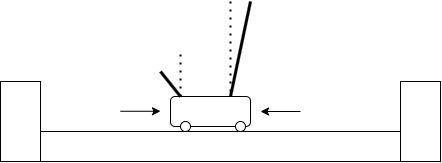
\includegraphics[width=0.5\textwidth]{images/pole_balancing.drawio.png}
    \caption{Ilustrație a problemei double pole balancing. Scopul unui algoritm in cadrul acestui mediu este să miște platforma astfel încât pilonii de pe ea sa nu se răstoarne}
    \label{fig:double_pole}
\end{figure}

Totuși, aceeași problema a fost rezolvat de 5 ori mai rapid de \textbf{Enforced Subpopulations}(ESP)\cite{ESP}, astfel că autorii NEAT si-au propus sa demonstreze un argument mai puternic pentru evoluția structurilor, anume ca modificând atât topologia cat și ponderile putem spori cu mult performanta algoritmilor NE. NEAT poate face asta datorita faptului ca minimizează structurile rețelelor pe tot parcursul algoritmului. 
Au existat pe parcursul timpului mai multe metode de evoluție atât pentru topologiile cat și ponderile rețelelor neuronale, ale căror ideii autorii le-au unit în \cite{NEAT} sub termenul de \textbf{"TWEANS"}(Topology and Weight Evolving Artificial Neural Networks). Pentru dezvoltarea NEAT, Kenneth O. Stanley a adresat un număr de probleme nerezolvate la clasa de algoritmi TWEANS. Înainte de asta ar trebui totuși sa prezentam cum funcționează rețelele neuronale și cum acestea învață.

\section{Rețele Neuronale Artificiale}
În natura, o rețea neuronala reprezinta o rețea de neuroni interconectați, care sunt responsabili de funcționarea sistemului nervos. 
Sunt specializați în transmiterea informației prin semnale electrice și au 4 componente principale, dendritele, corpul celular, axonul și butonii terminali.
\begin{figure}[h]
    \centering
    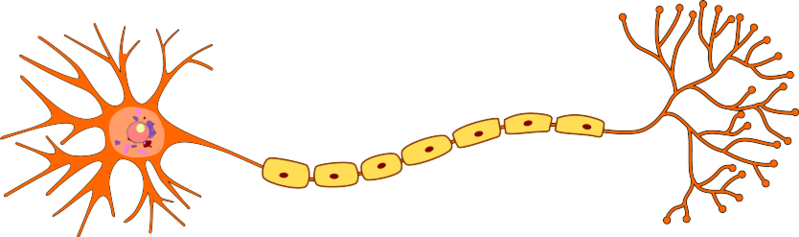
\includegraphics[width=1\textwidth]{images/neuron_structure.png}
    \caption{Structura unui neuron.\cite{Neuron}}
    \label{fig:neuron}
\end{figure}
Fiecare neuron primește informația prin dendrite și le transmite prin axon printr-un semnal electric cu toată puterea sa, dacă a primit destulă informație prin Dendrite. Neuronii sunt conectați intre ei prin sinapse, iar sinapsele își pot adapta numărul de receptori pentru a controla puterea semnalului care vine de la un neuron.
O rețea neuronala artificiala este compusa dintr-o serie de noduri conectate intre ele ca un graf. 
Ca structura, o rețea are un strat de noduri de intrare și  unul de noduri de ieșire, și opțional un număr de straturi ascunse în cadrul rețelelor neuronale profunde.
Fiecare conexiune are o pondere asociata ei ce reprezintă puterea conexiunii. 
Aceste ponderi se pot adapta astfel încât rețeaua sa funcționeze conform așteptărilor. Conform Teoriei Aproximării Universale, o rețea neuronala ar putea sa ajungă aproape de a aproxima orice funcție pentru care este adaptată.
Spre deosebire de creier, într-o rețea neuronala pot exista mai multe tipuri de neuroni, determinați de o funcție de activare. Dacă nu folosim o funcție de activare, valoarea unui neuron este reprezentata de o suma ponderata a intrărilor(Formula \ref{eq:sumaPonderata}) plus opțional un bias al neuronului.

\begin{equation}\label{eq:sumaPonderata}
    z = \sum_{i} w_i x_i + b
\end{equation}

Dacă este folosita o funcție de activare, atunci semnalul nodului va fi outputul funcției de activare, iar input-ul este suma ponderata dintre conexiunile și intrările nodului.
\begin{figure}[h]
    \centering
    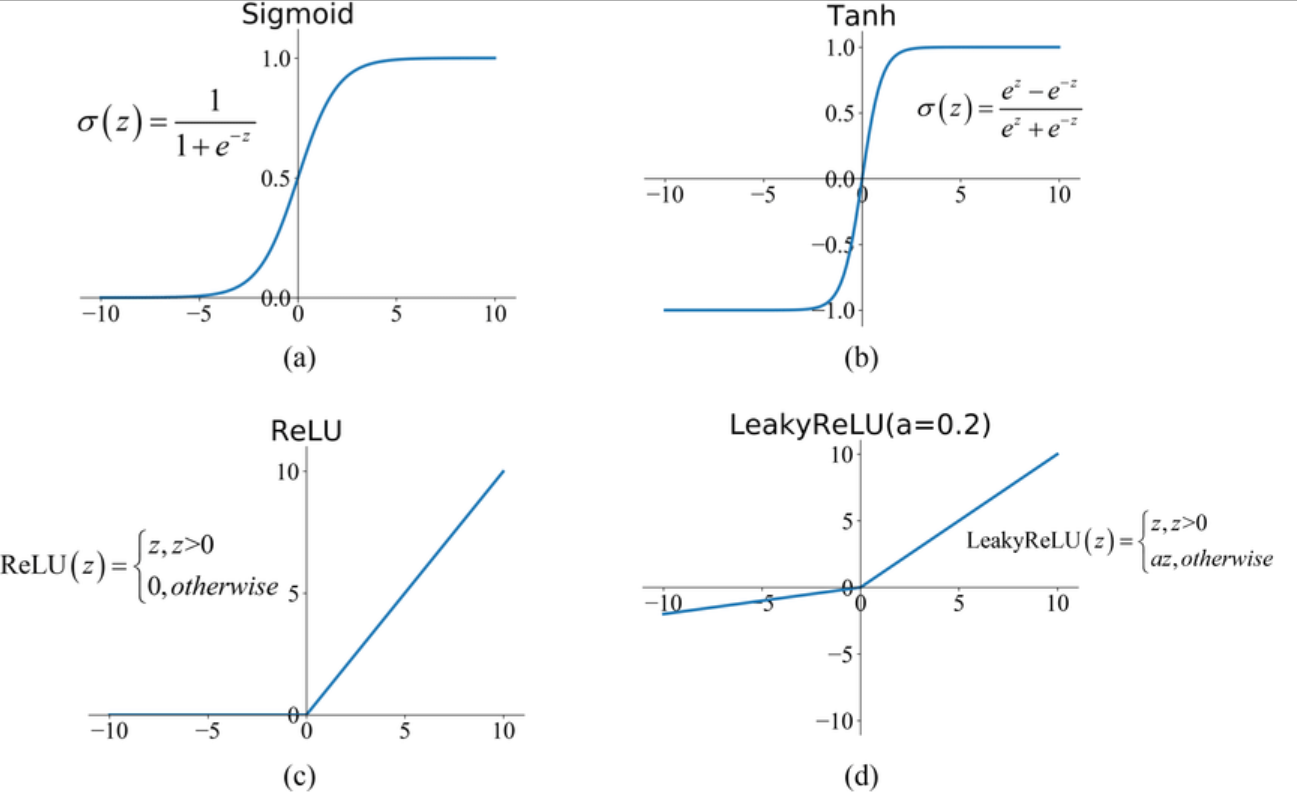
\includegraphics[width=1\textwidth]{images/activation_functions.png}
    \caption{Funcții de activare comune: (a) Sigmoid, (b) Tanh, (c) ReLU, and (d) LReLU.\cite{activation_functions}}
    \label{fig:neuron}
\end{figure}

Rețelele neuronale artificiale tradiționale sunt feedforward, adică datele sunt procesate într-o singura direcție, de la input la output, iar învățarea se face prin algoritmul de backpropagation.
În documentul care descrie NEAT, nu sunt expuse restricții asupra conexiunilor care se pot forma, deci algoritmul poate duce la generarea rețelelor neuronale recurente.
Acestea pot procesa date secvențiale, deoarece conțin conexiuni ciclice, ce se pot forma intre oricare noduri, inclusiv nodul de la care conexiunea a pornit. La fiecare pas de timp, în RNN nodurile procesează atât intrarea curenta cat și ieșirea nodului recurent anterior, ceea ce permite rețelei sa utilizeze informații din trecut.
Pentru antrenare NEAT nu folosește backtracking, ci operatorii genetici.

\section{Problemele în TWEANNs și inovațiile în NEAT}
\subsection{Codificare}\label{Codificare}
O problema pe care trebuie sa o rezolve orice TWEANN este modul în care specificam genomul unui individ. Aici sunt doua categorii mai mari, \textbf{codificare indirecta}  și \textbf{directa}.
Codificarea indirecte de obicei doar specifica reguli pentru crearea fenotipului, și sunt specifice algoritmilor care le folosesc
Pentru codificarea directa opțiunile sunt \textbf{codificarea binara}, care folosește codificare clasica a grafurilor cu șiruri de biți, precum "Structured Genetic Algorithm"(sGA)\cite{sGA}, care reprezinta prin șiruri de biți matricea de conexiuni a rețelei, însa cele mai întâlnite codificări sunt cele de tip graf, care reprezinta grafurile în mod mai explicit.
NEAT folosește o codificare directa, din cauza ca codificările indirecte neavând o mapare directa la fenotip, dacă nu suntem foarte familiari cu procesele genetice, pot perturba căutarea în moduri impredictibile și greu de detectat. Codificarea pe care o alegem este foarte importanta, deoarece aceasta afectează costul operației de crossover, astfel ca exista TWEANNs "nonmating", care nici măcar nu folosesc acest operator\\
Codificarea NEAT a fost proiectata cu scopul de a permite alinierea genom-urilor pentru crossover fără a fi nevoie de o analiza costisitoare a topologiei. Aceasta codificare este reprezentata de o lista de node genes, și o lista de connection genes. Pentru fiecare node gene este specificat id-ul sau și tipul de nod, care clasifica nodurile în noduri de intrare, de ieșire, si noduri ascunse. Primele sunt nodurile de intrare, după care cele de ieșire iar cele hidden sa adaugă la capătul listei în urma mutațiilor.
Fiecare conection gene conține: un in-node și un out-node, care exprima nodurile și direcția conexiunii, ponderea asociata cu conexiunea, o valoare boolean care indica dacă conexiunea ar trebui sa fie exprimata în fenotip, și un număr de inovație(prezentam de ce este necesar în secțiunea \ref{Numar de inovatie}), care permite găsire genelor care corespund din diferiți indivizi și e una din piesele centrale ale algoritmului.
\begin{figure}[h]
    \centering
    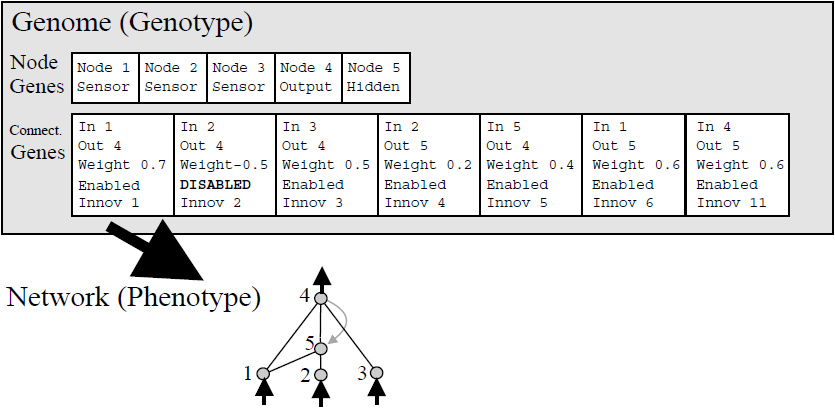
\includegraphics[width=1\textwidth]{images/genotip_fenotip_neat.png}
    \caption{Genotipul in cadrul NEAT si fenotipul(rețeaua neuronala) pe care acesta îl exprima. Figura 2 din \cite{NEAT}},
    \label{fig:encoding}
\end{figure}

\subsection{Inițializarea populației}\label{InitializareNeat}
La majoritatea algoritmilor din clasa TWEANN, populația inițiala este generata cu topologii aleatorii, pentru a asigura diversitate în structurile rețelelor. Totuși, inițializare în modul asta produce multe probleme pentru TWEANNS:
\begin{enumerate}
    \item Nu avem nici o garanție ca informația poate ajunge din fiecare intrare la fiecare ieșire, ceea ce poate face ca unele intrări sa fie irelevante. Timp important de procesare va fi pierdut pentru a scăpa de astfel de rețele.
    \item Ideal am dori ca soluțiile obținute sa fie minime, adică un număr minim de noduri și conexiuni, deoarece o rețea mai complexa necesita mai mult timp pentru optimizarea ponderilor. Cu inițializarea aleatorie, o mare parte din timp ar fi folosita pentru filtrarea structurilor extra care nu ar fi trebuit sa existe de la început. Evaluarea relelor mai complexe ia mai mult timp, dar prin aceasta inițializare nu avem nici o garanție ca soluția va fi minima, deoarece orice rețea atâta timp cat are un fitness mare poate domina peste celelalte.
\end{enumerate}

Soluția NEAT este sa înceapă în mod minim. Populația inițiala are fiecare nod de intrare conectat cu cele de ieșire cu ponderi aleatorii, și nici un nod ascuns, astfel soluția va adăuga structuri noi doar atunci când aceste ajuta la îmbunătățirea fitness-ului. Astfel se asigura minimalitatea nu doar la final dar pe parcursul tuturor generațiilor. Ar trebui sa precizam ca inițial, adăugând unei rețele structuri noi, care nu au fost optimizate, va face ca fitness-ul sa scadă inițial, deci indivizii cu inovații topologice sunt la risc sa dispară, asta fiind un alt motiv pentru care majoritatea algoritmilor TWEANN folosesc inițializarea cu topologii aleatorii. Pentru a evita pierderea inovațiilor, NEAT folsește \textbf{"Speciația"}, pe care o vom detalia în secțiunea \ref{Speciatie}.

\subsection{Problema convențiilor concurente și numerele de inovație}\label{Numar de inovatie}
Problema convențiilor concurente apare atunci când exista mai mult de un singur mod de a reprezenta o rețea neuronala optimizata pentru o problema.
Crossover în cazul a doua astfel de soluții poate duce la pierderea de informație în cadrul noului copil format.
Aceasta problema este încă mai grava în cadrul TWEANNs, deoarece soluții pentru o problema pot fi reprezentate prin topologii complet diferite, iar genomul fiecăreia poate avea lungimi diferite, agravând problema convențiilor concurente. 
Soluția în cadrul NEAT la aceasta problema este inspirata din soluția naturii în cadrul reproducerii sexuale, adică \textbf{omologia}, doua gene fiind omoloage dacă ele sunt trăsături ale aceleiași alele.
NEAT stabilește omologia dintre gene prin intermediul \textbf{marcatorilor istorici}, reprezentați de \textbf{numere de inovație}, care permit stabilirea originii istorice a unei gene, iar astfel putem identifica și genele omoloage.
Vom prezenta cum apar și cum sunt folosite numerele de inovație în secțiunile \ref*{OperatoriGenetici} și \ref*{Speciatie}

\subsection{Operatori Genetici}\label{OperatoriGenetici}
NEAT folosește 2 operatori genetici pentru modificarea genomul-ui indivizilor, mutația și crossover.
Prin mutație, ca și la ceilalți algoritmi de NE, se pot modifica ponderile, prin perturbarea lor sau prin asignarea unei noi valori aleatorii, însa pentru NEAT mutație este și modalitate prin care introducem schimbări structurale.
Sunt folosite 2 tipuri de mutație structurala, "add connection", prin care se adaugă o conexiune cu pondere aleatorie intre oricare 2 noduri care nu erau conectate deja, și "add node", care alege o conexiune în mod aleatoriu, și adaugă un nou nod în locul ei.
Mai exact, conexiunea aleasa este dezactivata, și se creează o noua conexiune intre nodul de intrare al conexiunii dezactivate și nodul nou creat, cu ponderea de 1, iar conexiunea dintre nodul nou și nodul de ieșire primește ponderea celei dezactivate.
Astfel se minimizează efectul inițial al modificărilor structurale, iar ponderile noilor conexiuni vor fi modificate în generațiile viitoare.

De fiecare data când producem o modificare structurala, fiecare gena de conexiune are adăugat și un nou număr de inovație din punct de vedere global.
Acest număr ne permite sa stabilim originea istorica a acestei gene.
Dacă în cursul unei generații, păstram o lista a inovațiilor care au avut loc iar în genomul a 2 indivizi diferiți va apărea o aceeași gena de conexiune, poate doar cu ponderi diferite, aceste gene vor primi ambele același număr de inovație, pentru ca reprezinta aceeași structura dar care a apărut în mod independent în cadrul fiecăreia.
Crossover reprezinta încrucișarea genomului celor 2 părinti, pentru a crea un copil ce are structuri din partea ambilor
Acum, datorita marcatorilor istorici, în cadrul crossover doua genomuri pot fi aliniate după genele care au numere de inovație egale, acestea sunt gene "matching".
Genele care nu sunt matching sunt fie "disjoint" dacă sunt în limita numerelor de inovație a ambilor părinti, fie "excess" dacă unul din părinti are numere de inovații mai mari decât cel mai mare număr al celuilalt părinte.
\begin{figure}[h]
    \centering
    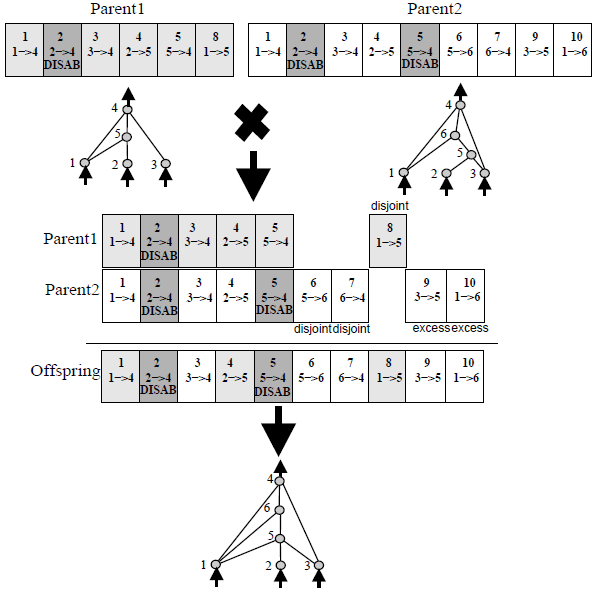
\includegraphics[width=1\textwidth]{images/crossover_matching.png}
    \caption{Procesul de "matching" pentru doua genomuri diferite. Reprezinta figura 4 din \cite{NEAT}}
    \label{fig:crossover}
\end{figure}
În cadrul compunerii copilului, acesta moștenește în mod aleator genele parching ale ambilor părinti, însa doar genele disjoint și excess ale părintelui cu cel mai mare "fitness".
În cazul în care ambii părinti au fitness egal, atunci și genele excess și disjoint sunt moștenite aleator.
Pentru genele dezactivate, este o probabilitate prestabilita ca o gena sa rămână dezactivata dacă ea e asa în cadrul oricăruia dintre părinti.
\\
Prin intermediul acestor 2 operatori genetici, este introdusa diversitate în cadrul populației.
Totuși, de obicei, datorita faptului ca structurile mai mici au mai puține conexiuni, aceste se pot optimiza mai rapid, iar adăugarea de noi structuri, pana acestea sunt optimizate, va scădea din fitness-ul rețelei, deci inevitabil noile inovații ar dispărea rapid dintr-o populație normala, cu tote ca potențial ele ar fi chiar necesare.
Din acest motiv în NEAT este nevoie de \textbf{Speciație}, pe care o prezentam în secțiunea \ref*{Speciatie}.

\subsection{Speciație}\label{Speciatie}
Speciația este un mod de a proteja noile inovații topologice apărute.
Ideea este de a permite indivizilor sa concureze în propria lor nișă, nu cu întreaga populație.
Pentru a detalia, topologiile similare din cadrul populației vor fi încadrate în specii, organismele din aceleași specii concurează în mod principal intre ele, și astfel au timp sa își optimizeze conexiunile.
Cum anume sunt determinate speciile și organismele din cadrul lor? Tot cu ajutorul numerelor de inovație. 
Numărul de gene "desjoint" si "excess" sunt un indicator bun al distantei din punct de vedere al compatibilității intre 2 genomuri.
Astfel, autorii NEAT au ajuns la o formula simpla care sa măsoare compatibilitatea ca o distanta intre 2 structuri diferite în NEAT(notam $\delta$) în termeni de număr de gene excess $E$ și număr de gene desjoint $D$, plus media diferenței dintre genele matching $\overline{W}$:

\begin{equation}\label{eq:compatibility}
    \delta = \frac{c_1 \cdot E}{N} + \frac{c_2 \cdot D}{N} + c_3 \cdot \overline{W} 
\end{equation}

Coeficienții $c_1$, $c_2$ si $c_3$ ajustează importanta acestor factori, iar $N$, care reprezinta numărul de connection genes a genomului cel mai lung, normalizează valorile conform dimensiunii genomului.
Prin calculul valorii $\delta$ putem desfășura procesul de speciație cu ajutorul unei valori stabilite în prealabil, pragul de compatibilitate $\delta_t$.
Procesul de speciație se desfășoară în următorul mod.
Fiecare specie are un genom care o reprezinta. Fie un genom $g$ din generația curenta, acesta este plasat în prima specie cu a cărui reprezentant este compatibil, adică  $\delta < \delta_t$.
Dacă nu exista nici o specie compatibila, se formează una noua cu $g$ ca reprezentat al acesteia.

\subsection{Reproducerea}\label{Reproducerea}
NEAT folosește un mecanism numit \textbf{"explicit fitness sharing"} pentru a evita ca o specie sa devina prea mare și sa ajungă de dimensiunea întregii populații.
Practic, toate organismele din aceeași specie împărtășesc fitness-ul speciei lor.
Fitness-ul ajustat al organismului $i$ este calculat prin formula:

\begin{equation}\label{eq:adjustedFitness}
    f\prime_i  = \frac{f_i}{\sum_{j = 1}^{n}sh(\delta(i,j))}
\end{equation}

unde $f\prime_i$ e fitness-ul ajustat al individului $i$, $n$ e numărul de organisme din populație, iar funcția $sh$ are valoare 0 când $\delta(i, j)$ este peste $\delta_t$, dar 1 altfel.
Astfel, partea de jos a fracției reprezinta doar numărul de indivizi din aceeași specie cu organismul $i$.
Fiecărei specii ii este acordat un număr diferit de membri potențiali depinzând de suma a $f\prime_i$ a membrilor speciei După formula:
\begin{equation}\label{eq:potentialMembers}
    n_k = \frac{\overline{F_k}}{\overline{F_{tot}}} |P|
\end{equation}
unde $k$ reprezinta o specie, $n_k$ e nr de membri asignați speciei, $|P|$ este numărul de indivizi în populație, $\overline{F_k}$ este media fitnessului speciei, adică $\overline{F_k} = \sum_{i}^{} f\prime_i$, iar $\overline{F_{tot}} = \sum_{k}^{} \overline{F_k}$
Întreaga populație este apoi înlocuită de copii membrilor mai buni ai fiecărei specii, membrii mai slabi fiind eliminați în prealabil.
Scopul final al speciației este protejare inovațiilor topologice, iar sistemul întreg cauta o soluție în cel mai rapid mod posibil, deoarece inovații noi apar și sunt păstrate doar atunci când e necesar.
